
%%%%%%%%%%%%%%%%%%%%%%%%%%%%%%%%%%%%%%%%%%%%%%%%%%%%%%%%%%%%%%%%%%%%%%%%%%%%%%%%

%        1         2         3         4         5         6         7         8

\documentclass[letterpaper, 10 pt, conference]{ieeeconf}  % Comment this line out if you need a4paper

%\documentclass[a4paper, 10pt, conference]{ieeeconf}      % Use this line for a4 paper

\IEEEoverridecommandlockouts                              % This command is only needed if 
                                                          % you want to use the \thanks command

\overrideIEEEmargins                                      % Needed to meet printer requirements.


\usepackage{graphics} % for pdf, bitmapped graphics files
\usepackage{epsfig} % for postscript graphics files
\usepackage{mathptmx} % assumes new font selection scheme installed
\usepackage{times} % assumes new font selection scheme installed
\usepackage{amsmath} % assumes amsmath package installed
\usepackage{amssymb}  % assumes amsmath package installed

\usepackage[font=small,labelfont=bf]{caption}

% Other package
\usepackage{tikz}
\usepackage{graphicx}
\usepackage{caption} 
\usepackage{subcaption}
\usepackage{multirow}
\usepackage{array}
\usepackage{booktabs}
\usepackage{hyperref}

\usepackage{pdfpages}
\usepackage{caption}
%\usepackage{geometry}
\usepackage{import}
\usepackage{standalone}

\title{\LARGE \bf
  Team-JSK: MBZIRC Progress Report 2
}
\author{\textbf{Team JSK} ({\texttt{www.jsk.t.u-tokyo.ac.jp}})% <-this % stops a space
  \\ JSK Lab, Graduate School of Information Science and Technology,
  The University of Tokyo \\
  7-3-1 Hongo, Bunkyo-ku, Tokyo, Japan 113-8656.  \\
}

\begin{document}

\maketitle
\thispagestyle{empty}
\pagestyle{empty}


\section{INTRODUCTION}
This document provides the second report of 
Team JSK's progress in preparing
for the Mohamed Bin Zayed International Robotics Challenge
(MBZIRC). The document highlights some of the advances made since the submission of the first progress report as well as future plans leading to the actual challenge. 


\section{PROJECT PERSONNEL}
Team JSK is currently made up of 13 members: Prof. Masayuki Inaba, Prof. Kei
Okada, Dr. Yohei Kakiuchi, Dr. Wesley Chan, Bakui Chou, Xiangyu Chen,
Krishneel Chaudhary, Kohei Kimura, Yuki Furuta, Hiroto
Mizohana, Fan Shi and Tomoki Anzai. The team is roughly divided into
three groups corresponding to each task with groups having overlapping
personnel.

\section{CHALLENGE 1: LANDING UAV ON A MOVING VEHICLE}

%Copyright (C) 2016 by Krishneel@JSK Lab, The University of Tokyo

%Copyright (C) 2016 by Krishneel@JSK Lab, The University of Tokyo

\documentclass{standalone}
\usepackage{footnote}
\usepackage{hyperref}
\usepackage{graphicx}
\usepackage{fancyhdr}

\renewcommand\footnoterule{%
  \kern-3\p@
  \hrule\@width2.5cm
  \kern2.6\p@
}
\makeatother

\begin{document}

\subsection{Platforms}
We customized the DJI developer platform M100 as shown in Fig.\ref{figure:task1-platform} (top). We used two Nvidia Jeston TX1 to distribute the heave computation load required for image processing. The two processors are connected via a wired internal network.
We also employed a camera with fisheye lens that has a $250^\circ$ wide viewing angle for tracking, as well as optical-flow $\&$ sonar sensor units to estimate the ego-motion of the UAV. The system framework is shown in Fig.\ref{figure:task1-platform} (bottom). The processing nodes inside the processors will be explained below.

\begin{figure}[h]
    \begin{center}
        \begin{minipage}{\hsize}
          \begin{center}
      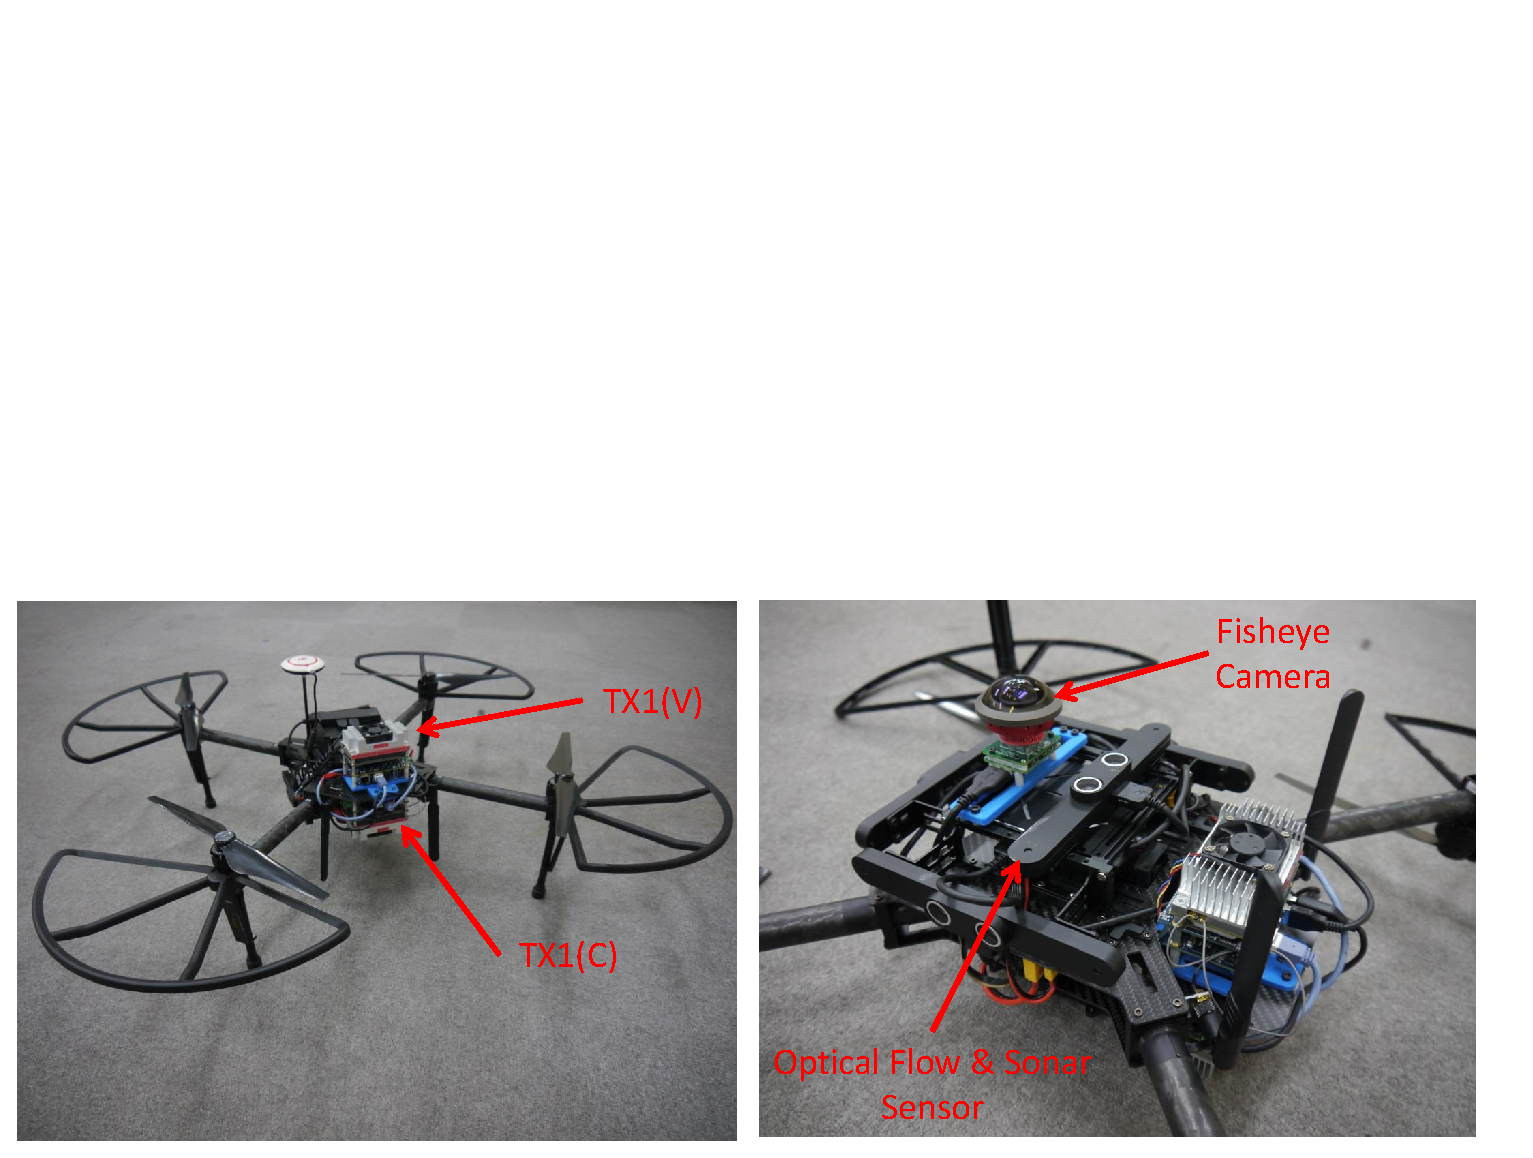
\includegraphics[clip, bb= 0 0 700 260, width=\columnwidth]{sections/task1/images/task1_hardware.eps}
          \end{center}
        \end{minipage}
        \begin{minipage}{1.0\hsize}
          \begin{center}
      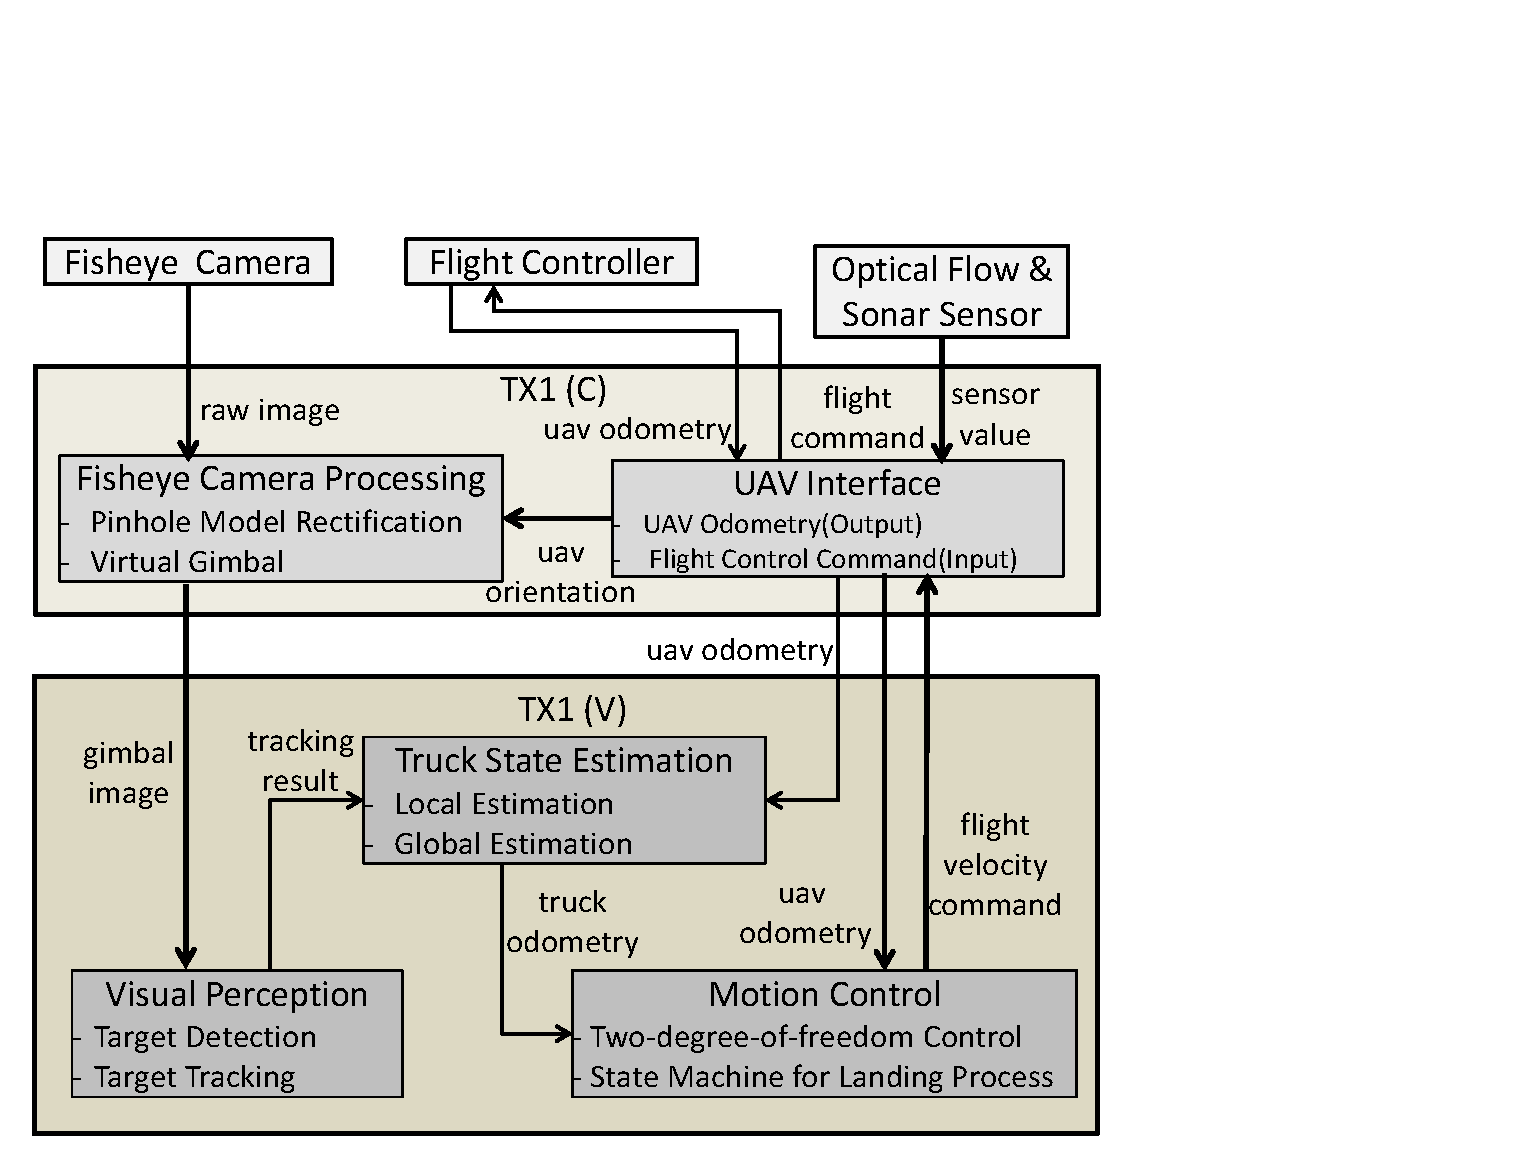
\includegraphics[clip, bb= 0 0 525 440, width=0.9\columnwidth]{sections/task1/images/task1_framework.eps}
          \end{center}
        \end{minipage}
    \end{center}
    \caption{Top: hardware platform DJI M100. Bottom: system diagram of the platform.}
    \label{figure:task1-platform}
\end{figure}


\subsection{Software Environment}
The visual perception algorithms and motion control are implemented
on Robot Operating System (ROS) environment\footnote{\url{http://www.ros.org}}.
We used Gazebo\footnote{\url{gazebosim.org}} for virtual simulations
\footnote{\url{https://github.com/start-jsk/jsk_mbzirc}}. Our
algorithms are implemented in C/C++, Python and CUDA-C.


\subsection{Visual Perception}

Image processing is one of the fundamental component of autonomous
systems. With efficient and robust image processing, planning and
decision making can be done more readily which improves the accuracy
and robustness of the execution of the assigned task. Hence, one of our
primary objective while designing our software architectures was
real-time performance with minimal loss of accuracy in image processing. The visual
component of task 1 includes three main stages described as follows:

\subsubsection{Fisheye Camera Processing}
To perform image processing using the images obtained from the fisheye camera, we first convert the raw images into pinhole model images. Furthermore, we also developed an original method called virtual gimbal, which combines the orientation data of UAV with the raw image data to calculate a stabilized image frame (Fig.\ref{figure:fisheye-virtual-gimbal}). This method is crucial when the UAV tilts with a large angle (e.g. greater than $20^\circ$) while tracking the downward target.

\begin{figure}[h]
    \begin{center}
      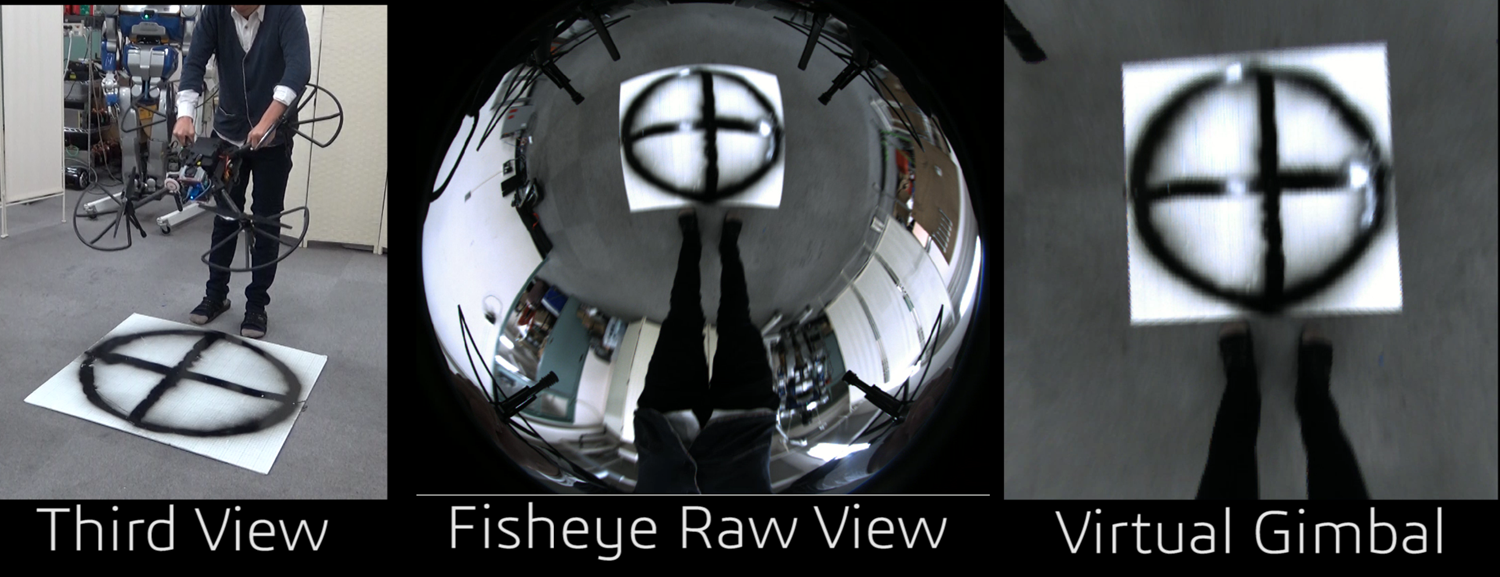
\includegraphics[width=0.9\columnwidth]{sections/task1/images/fisheye_virtual_gimbal.png}
    \end{center}
    \caption{Fisheye Virtual Gimbal}
    \label{figure:fisheye-virtual-gimbal}
\end{figure}

\subsubsection{Target Detection}
The target detection phase is the initial localization of the landing
region (heliport) on the truck. To detect the heliport we use a
traditional computer vision detection approach where by a sliding
window based method is used. However such raster scanning windows are
computationally expensive even for high end systems. To overcome this
crucial limitation we first generate candidate object
regions. Since the heliport is fixed to a moving target, we use
Gaussian based background subtraction fused with Kalman Filters for 
global motion compensation to generate regions of interest
(ROI)  with stable changes. The candidate ROI's are then ranked using
edge similarity between each sliding window. High scoring ROI are then
used for detecting the heliport using a pre-trained detector. 
In the following, let $\mathbf{H}$ denote the detected target region.

\subsubsection{Target Tracking}

In order for an UAV to approach and land on the heliport, online visual
feedback is very important since the target is constantly moving.
Using the assumption that the target is not
expected to change abruptly both in terms of visual motion and
appearances, we use visual tracking for online feedback.
The detected region $\mathbf{H}$ is used to initialize the
tracker. Our visual tracking algorithm is highly efficient and robust
to both scale and visual changes and runs in real time. Thus, it provides frame by frame location of the target. To enable a tracker
to run online in real time, we carefully crafted the expensive process
of feature computation by reducing it to a one time process. 
The invariant features for tracking are computed by passing the image
through several pre-trained kernels of varying dimensions. By varying
the sizes of the kernel, an approximate scale can also be detected.
Furthermore, the tracker is updated online at fixed intervals.

\begin{figure}[t!]
  \centering
  \includegraphics[height=1in]{sections/task1/images/detect2}
  \includegraphics[height=1in]{sections/task1/images/detect1}
  \caption{Illustration of truck and heliport detection.}
\end{figure}

\subsection{Truck State Estimation}

We can obtain the relative pixel position of a target object in the fisheye camera's image with the help of our visual perception algorithm. Furthermore, the UAV's state , including flying height, velocities, and rotation angles, can be obtained from sensors on the UAV. Using these information, the speed of target object in world coordinate can be calculated. Finally, with a low-pass filter's help, we can obtain a fairly accurate estimation of target velocity.

\subsection{Motion Control}

\subsubsection{Two-degree-of-freedom Control}

We present a two-degree-of-freedom control method including both feedforward and feedback method for truck tracking. Using the approach described in the previous section, a good estimation of the truck velocity can be obtained and used by a feedforward algorithm. Then, a PI controller can be used to make gentle adjustments to help the UAV maintain a position above the truck.

\subsubsection{State Machine for Landing Process}

We carefully designed a state machine for the landing process. We defined an inverted conical region relative to the center of the tracking object. When UAV is stably moving in this region, UAV is considered to be tightly keeping track of the moving object, and the UAV is allowed descend with a stable speed. Our strategy is that once the UAV is within 0.35[m] above the truck, we will stop its gradual descend and adjust the UAV's position to the center of the heliport and land directly and quickly to it. The reason is that currently our visual tracker detects the inside circle region of the heliport, whose radius is 0.5[m], and the fisheye camera we use has a $120^\circ$ viewing angle. This means that when the UAV is less than 0.29[m] above the heliport, the camera would not be able to see the whole heliport. 0.29[m] is a close enough distance for the UAV to land directly, and our experiments also proved that this strategy is feasible and practical.


\subsection{Results Achieved to Date}

We have completed the entire task one autonomously, landing on the 
target moving at 5[km/h], 10[km/h], and 15[km/h]. Moreover, we have demonstrated the effectiveness of our real time planning and tracking by showing the results of long duration
following of the target at over 35[km/h]. The results of these tracking and landing motion are shown in the progress video.

For landing control, we first tested our method to land on a static truck, and result shows that precision is within 10 centimeters, which is close to the results of a state-of-the-art work by HKUST's team who presented in ICRA2015. For a moving target, we succeeded in landing on the truck moving at 15[km/h] as shown in Fig.\ref{figure:landing}.

\begin{figure}[h]
    \begin{center}
      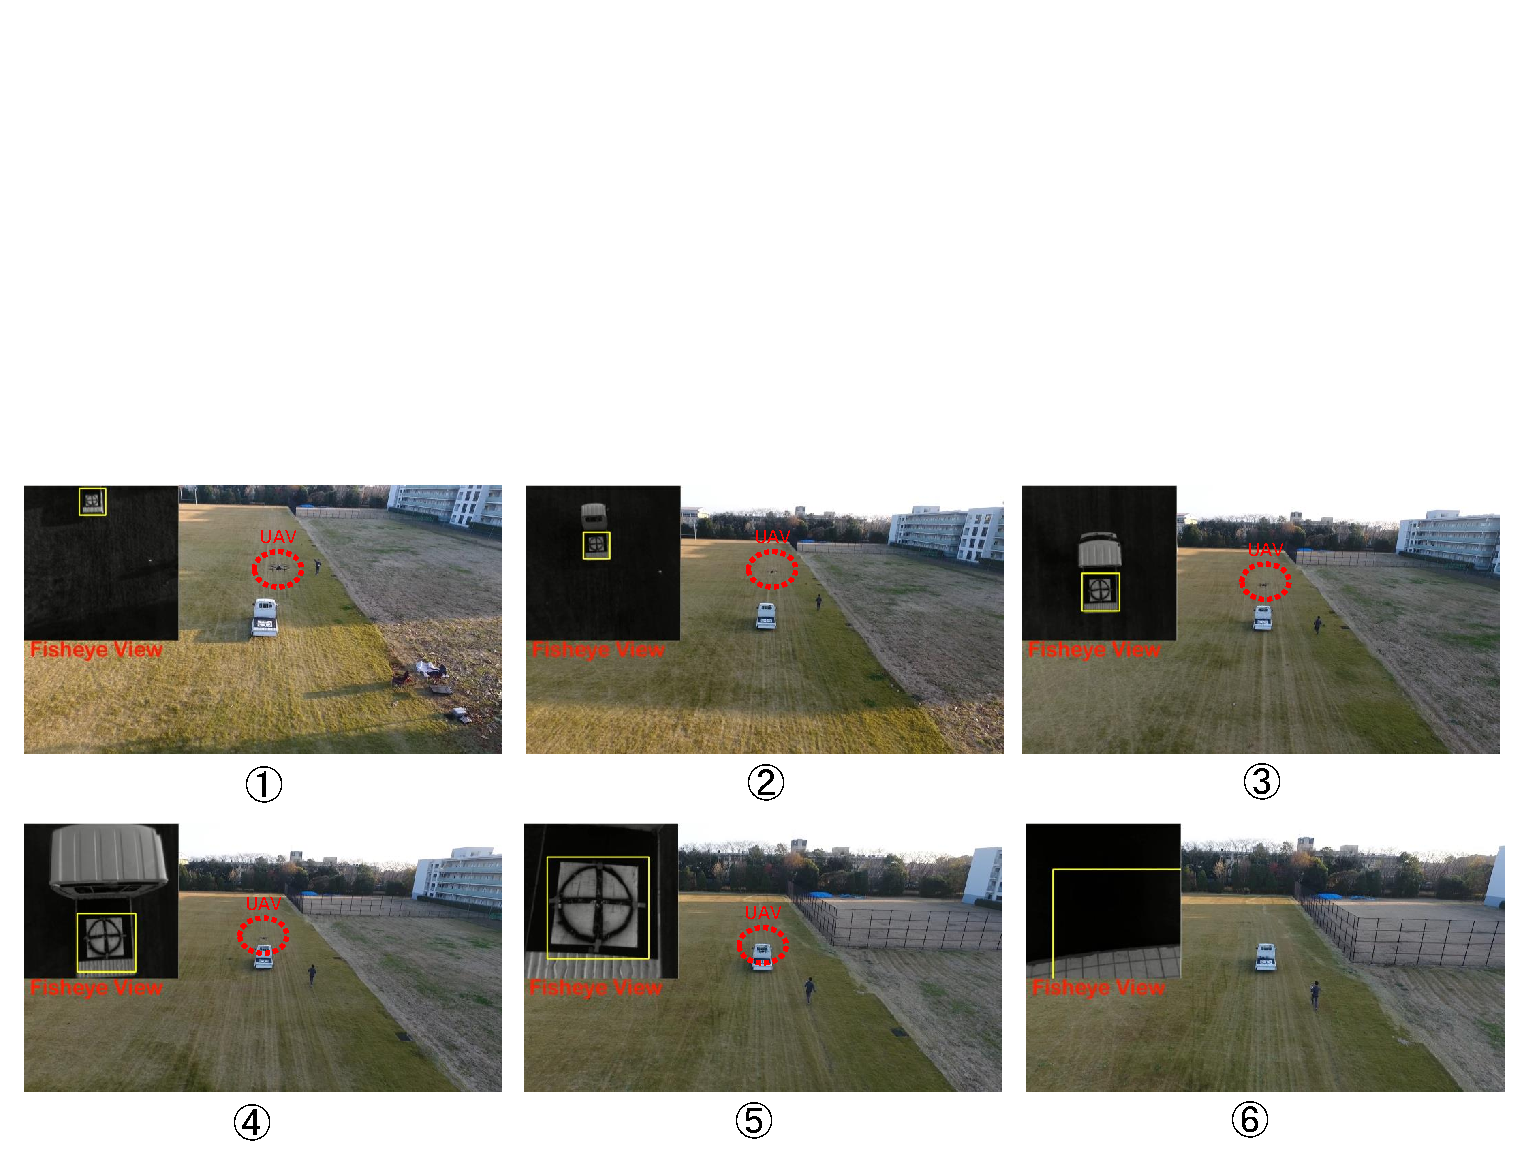
\includegraphics[clip, bb= 0 0 720 315, width=1.0\columnwidth]{sections/task1/images/task1_landing.eps}
    \end{center}
    \caption{The landing process in the case of [15km/h]. For more details, please see our video.}
    \label{figure:landing}
\end{figure}


\subsection{Future Work}
\subsubsection{Vision Algorithm}
Few improvements are required to increase the robustness of our
vision algorithms. First, we will add tracker drift recovery mode to
the visual tracking algorithm. Drift recovery will enable the
tracker to recover from drifting effects that may result from
occluded or lost target. Second, with the implementation of drift
recovery, we want the tracker to constantly update instead of updating at fixed
intervals. Such updating scheme will enable the tracker to adapt to
online visual changes without a need of prior learning.


\subsubsection{Landing Control}
Since outdoor landing when the target object is turning at a high speed is an unsolved difficult problem, currently our landing is also restricted in straight-road landing. However in the challenge, starting from the center crossroad, only a 20[m] straight road is available. Considering that the truck is moving at 15[km/h] (4.2[m/s]), the UAV has to land within 5[s]. Currently for development and safety consideration, our landing is slow and needs around 15[s].
In the next stage, we plan to re-evaluate these academic problems and make pioneer trails to generate realtime landing trajectories for landing then the target object is turning at a high speed.


\end{document}


%% insert yout latex module file here. the contents should go to the
%% tasks folder under section


\section{CHALLENGE 2: OPERATING A VALVE STEM}
\documentclass{standalone}
\begin{document}

\subsection{Hardware}

\documentclass{standalone}


\begin{document}

\subsubsection{New Gripper Design}
\documentclass{standalone}
\begin{document}

In our previous progress report, we described an approach where the robot rotated the valve stem by fitting the wrench head onto the shaft, then solving the inverse kinematics (IK) and moving its arm in a circular trajectory constrained to a plane parallel to the panel surface.
Due to joint limits of the robot, the IK for the trajectory may
not be solvable at certain arm positions. To reduce the chance of encountering unsolvable IK, we turned the wrench $90^{\circ}$ at a time, solving for a quarter circle trajectory's IK, and turn the valve stem four times. However, a drawback of this strategy is the time required to
complete the task. Thus, we designed a new gripper that uses the ring
end of the wrench, centered at the axis of rotation of the gripper servo
motor, by aligning and fitting the ring end to the valve
stem, and rotating the valve stem by rotating the gripper motor
$360^{\circ}$. Our new gripper is capable of rotating the valve 
stem with $5Nm$ of torque and complete the task without having
to solve for multiple IK's.

%% The last gripper in task 2 our humanoid robot have to fit the wrench
%% into the shaft and rotate $360$ degrees by move the arm and solve the
%% inverse kinematics. However, sometimes(usually) the inverse kinematics
%% can not be solved due to the limitation of the arm. In the first
%% report we attempt to rotate the wrench $4$ times with $90$ degrees
%% each time. This is very time consuming and now we designed a new
%% gripper that use the servo motor attached to the gripper which can
%% directly robot $360$ degrees and capable of the torque $5Nm$. 


Figure \ref{gripper} illustrates the new gripper which consists of a
servo motor and a magnetic attachment. We use a Dynamixel MX-106
servo motor which has a high stall torque of $8.4Nm$. At a payload of 
$5Nm$, the motor can still rotate at a speed of
more than $10 rpm$, thus, it allows our robot to complete turning 
the valve stem much faster.

%% To pick and align the wrench onto the shaft more reliably, the gripper is equipped with a spring-loaded attachment. When the wrench is picked by the robot, the spring push the central stick inside the ring end of the wrench to
%% ensure perfect alignment. The ring end of the wrench is used to
%% manipulate the shaft. To align the wrench to the shaft, only the
%% central stick needs to be aligned to the shaft. After alignment, the
%% gripper is pushed against the shaft which will result in the spring to
%% compress and the ring end of the wrench pushed into the shaft as shown
%% on the right in Fig.\ref{gripper}. The shaft is then easily rotated
%% using the Dynamixel motor.

%% FUTURE WORK
%% <<<<<<<<<<<<<<<<<
%% We need more experiments to validate the feasibility of
%% this gripper and then we can decide whether to equip this kind of
%% gripper in the final or not.
%% >>>>>>>>>>>>>>>>>>>>

 \begin{figure}%[hb]
    \begin{center}
    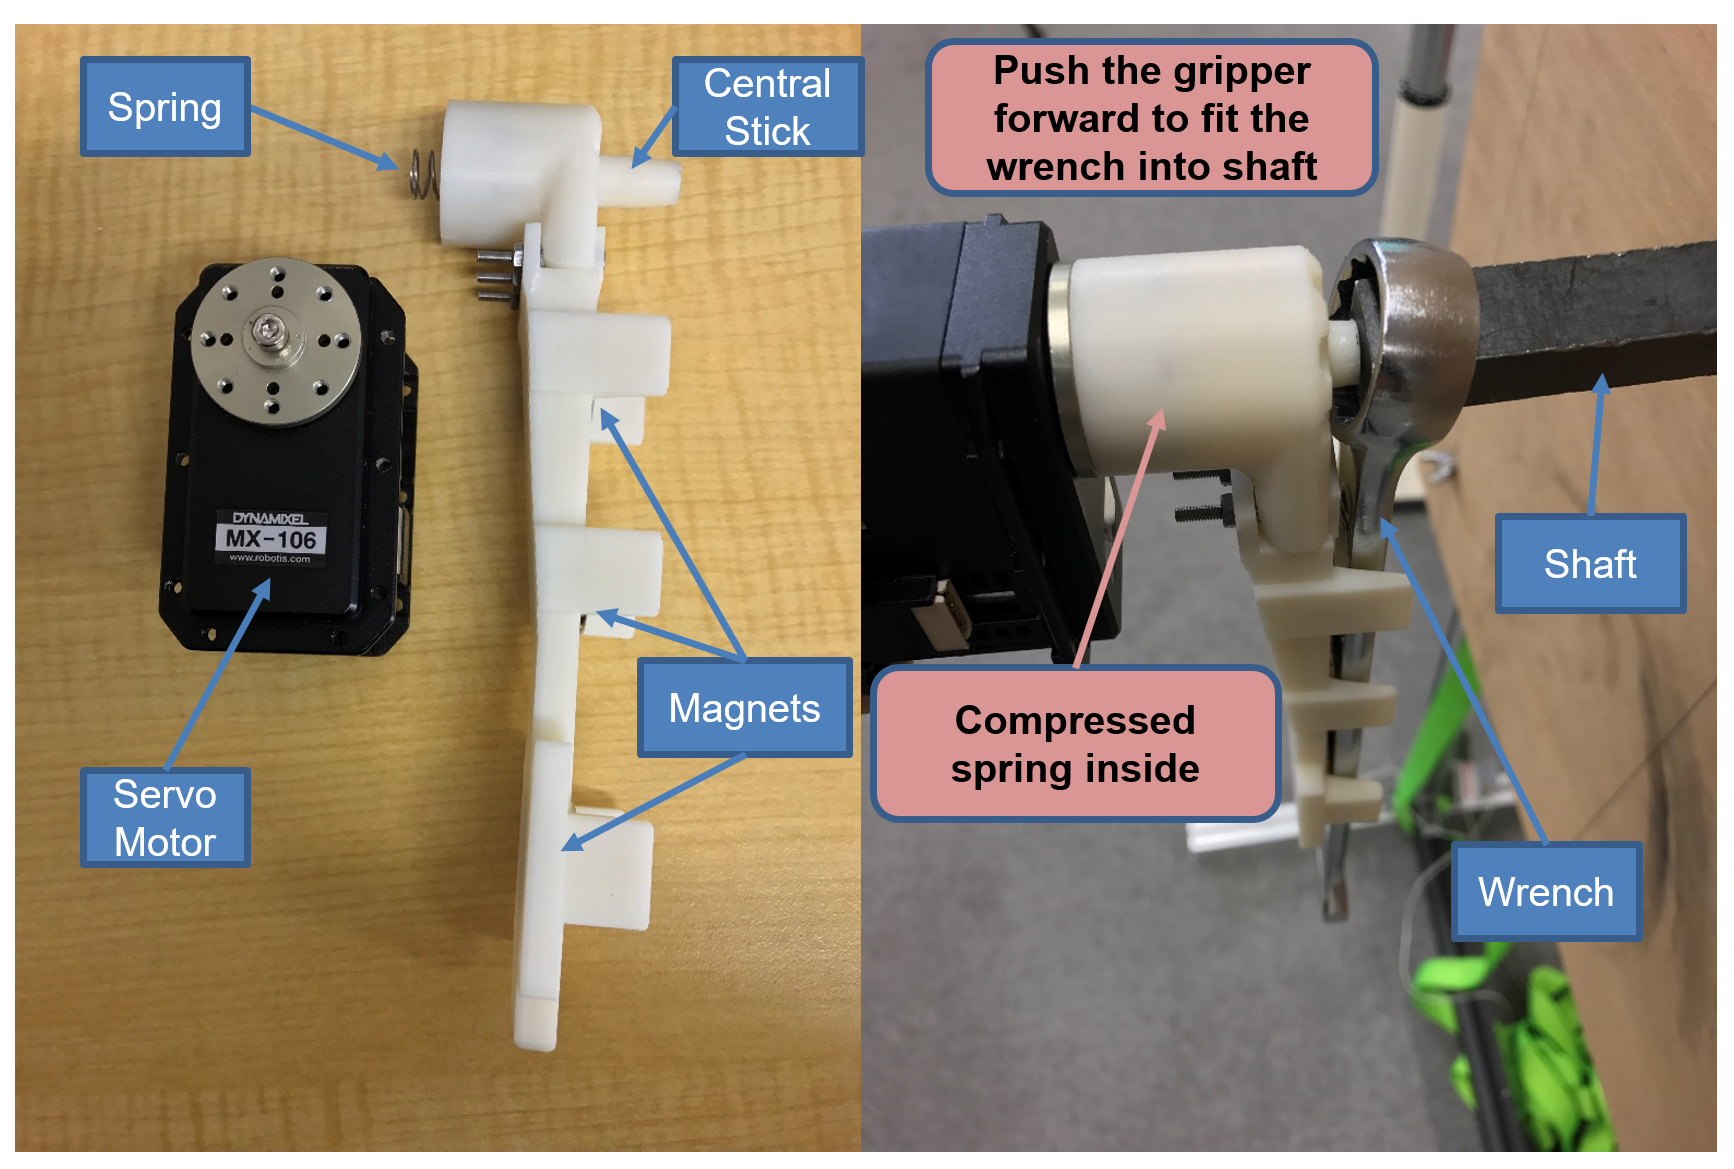
\includegraphics[keepaspectratio=true, width=1\linewidth,
      height=0.3\textheight]{sections//task2//images//gripper.png}
      \end{center}
    \caption{New Gripper Design}
    \label{gripper}
 \end{figure}

\end{document}


\subsubsection{New Robot Platform Aero}
\documentclass{standalone}

\usepackage{graphicx}
\usepackage{wrapfig}
\usepackage{lscape}
\usepackage{rotating}
\usepackage{epstopdf}

\begin{document}

We have been preparing a new robot platform, Aero (Fig.
\ref{fig:aero}), for use in task 2 of the challenge. From our past
experience (DRC Finals 2015), we encountered problems
with shipments. Transportation of large and heavy robots are
cumbersome, requires early shipment and difficult due to customs and
board control regulations of countries. 



% During DRC finals 2015, 
% From our past
% experience in DRC, transportation of large robots that require to be shipped
% separately proved to be very difficult due to customs regulations of
% countries. 

%% It is comparatively much easier to transport a robot that
%% can be carried onto an airplane with us as carry-on luggages. 
It is comparatively much easier to transport a robot that
can be separated into modules and taken onto an airplane with project personnel.
% with us as carry-on luggages. 
Aero is designed to be light weight and modular. Compared to 
our HPR2 robot we showed in our first progress report, which weighs
approximately 90 kg, aero only weighs approximately 65 kg. It is 
made up of a mobile base, a lifter, and an arm module, which can each 
be separated and fit into suitcases for transportation. 

%Aero contains 2 degrees of freedom in the lifter and 6 degrees of freedom in the arm. 

The lifter in the Aero has 2 degrees of freedom while the arm has 6 degrees
of freedom. For carrying out task 2, we have fitted Aero's arm
with the same magnetic gripper used for HRP2. 




We have been considering and testing several designs of the mobile base, including the following configurations:
\begin{itemize}
	\item 4 active Mecanum wheels 
	\item 4 active tire wheels
	\item 2 	active tire wheels + 1 passive caster wheel
	\item 2 	active tire wheels + 2 passive omni wheels
\end{itemize}

Each configuration trades off maneuverability, ease of path planing,
and compatibility with different terrains. Currently we are making our
next version of the mobile base, and we will select the best
configuration for our final design based on the competition arena
ground surface type. 


\begin{figure}[h]
   \newcommand \ilenght{0.1}
   \newcommand \iheight{2.0in}
   \newcommand \iwidth{0.46\textwidth}
   \centering
{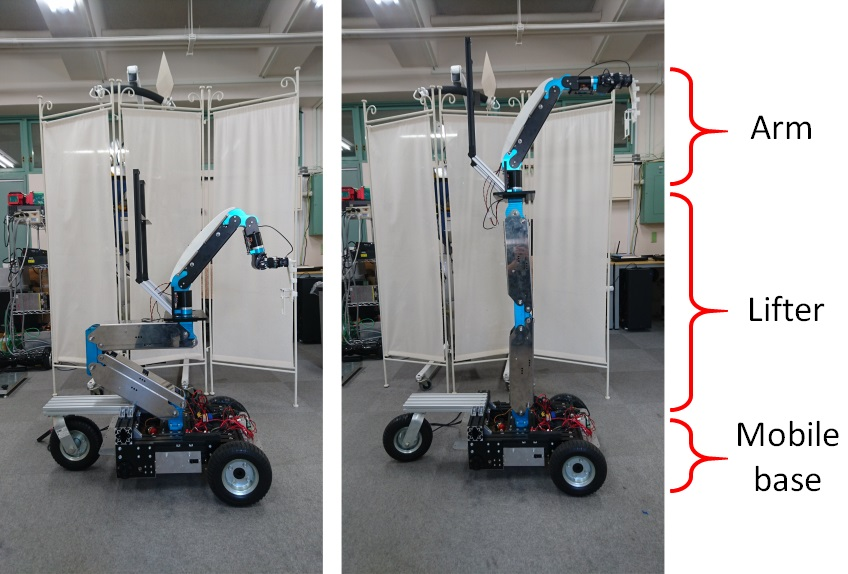
\includegraphics[width=\iwidth, height=\iheight]{sections/task2/images/aero.jpg}}\hspace{1.1em}%
   \caption{Our new robot platform, Aero. Left: lowered position. Right: extended position.}
   \label{fig:aero}
 \end{figure}

\end{document}


\end{document}


\subsection{Software}
\documentclass{standalone}

\usepackage{footnote}

\begin{document}

For our new robot Aero, we have created ROS wrappers for its low-level
controls and a Euslisp\footnote{\url{https://github.com/euslisp}}
model of it to enable the use of ROS and Euslisp, the same system we
used for HRP2. This allows us to use the same algorithms implemented
for HRP2 on Aero with minimal modifications. 


\end{document}

\subsection{General Approach}
\subsubsection{Navigation}
At first we tried to searching the panel by using long range laser sensor.
However, it was difficult to detect the panel because of the low density of points in long range.
So our second approach is running around the arena and searching the panel from pointcloud from the stereo camera.
When the panel is out of the range of stereo camera, the robot runs [run whole arena, I don't know good expression].
Then when the panel enter the range of stereo camera, the robot recognizes the panel by finding
the cluster of pointcloud which places about 1 meter height from ground and approach to the panel(Fig.\ref{fig: task2_panel-recognition}).
Finally, the robot runs around of the panel, recognizes it's the front side, then move to the front of the panel.

\begin{figure}[htb]
  \begin{center}
    \includegraphics[width=0.40\columnwidth]{sections/task2/nowprinting.png}
    \caption{Panel Recognition from Pointcloud}
    \label{fig: task2_panel-recognition}
  \end{center}
\end{figure}

\subsubsection{Wrench and valve stem recognition}
We detected the wrenches and valve stem in manually selected ROI in previous report. We could recognize
the length of the wrenches and the position of the wrenches and valve stem.

Our next target is autonomous recognition and recognition of the rotation
of the panel relative to the robot.
We find the plane from pointclound which is in front of the robot, then find the upper-right corner of the panel and calcurate the rotation.
The transform of the wrenches and valve stem is fixed, so we can easily detect the position and rotation of them(Fig.\ref{fig: task2_object-recognition}).

We experimented our recognition method and confirmed the accuracy of the recognition is enough.

\begin{figure}[htb]
  \begin{center}
    \includegraphics[width=0.40\columnwidth]{sections/task2/nowprinting.png}
    \caption{Wrenches and Valve Stem Recognition}
    \label{fig: task2_object-recognition}
  \end{center}
\end{figure}

\subsubsection{Picking the wrench}
We accomplished the wrench picking by just positioning the gripper to the detected wrench.

In order to improve the success rate, we are going to use handeye camera and image feedback control.


\subsubsection{Wrench fitting and turning}
We also accomplished wrench fitting and turning in previous report and are going to use handeye image feedback control.


\subsection{Results Achieved to Date}
\documentclass{standalone}
\begin{document}

\subsubsection{Hardware}
\documentclass{standalone}

\begin{document}

The lifter of Aero has gone through an upgrade once to increase its output and maximum reach in height. With its new lifter, the current version of Aero now has high enough output to rotate the valve stem at $5N/m$, and it is capable of reaching and turning the valve stem at the minimum possible height of the panel at $30cm$, as well as the maximum possible panel height at $100cm$.

We have created a teleoperating system for Aero, and using this system, together with code adapted from that we have created for HRP2, we have been able to successfully carry out the wrench picking and wrench turning part of task 2 with partial autonomy in an experiment. In our experiment, Aero begins standing in front of the panel. The operator aligns the arm with the wrench and pick up the wrench through teleoperation. After picking up the wrench, the operator then aligns the wrench with the valve stem, and fits the wrench onto it. Then, the robot autonomously generates a circular arc trajectory and execute it to turn the wrench.

\end{document}


\subsubsection{Software}
We accomplished Panel detection from the pointcloud of stereo camera and approaching to the panel automatically.

After approaching, our robot can detect the position and rotation of the wrenches and the valve stem also automatically.

Now we can navigate, recognize wrenches and valve stem, pick the correct wrench, fit the wrench to valve stem and rotate it in fully autonomous.




\end{document}

\subsection{Future Work}
\documentclass{standalone}
\begin{document}

\subsubsection{Hardware}
\documentclass{standalone}

\begin{document}

For our new gripper design, we will we conducting more tests to
determine how reliably the robot can fit the wrench onto the valve
stem and turn it. Regarding our new platform Aero, we are working
towards finalizing the
design of the mobile base at the moment. After we have built the new
version of the base, we will develop and test the controller
We will also be integrating camera and force sensor onto
the robot for perception. Furthermore, we will also need to finalized
our selection of on-board computers for Aero, design and build the
mount for them, and install them together with network capabilities to
make the system standalone and tether-free.


\end{document}


\subsubsection{Software}
Our future work in navigation includes searching for the panel within
the whole arena, detecting the front side of the panel, and finer
control of the robot position and orientation for alignment with the
panel for the task. Currently, the sizes of the wrenches are
determined by the length of the projected lines obtained from hough
transform. However, the accuracy of line estimation can vary based on
image intensity which can affect 
the recognition accuracy.
%recognition of wrench sizes.
 Therefore, we still need to detect the
size of the wrench head in order the determine the correct size
wrench with improved accuracy. Finally, we will be incorporating
the use of a handeye for performing visual feedback control to improve
picking and fitting of the wrench.




\end{document}



\end{document}

\section{CHALLENGE 3: SEARCH, PICK AND PLACE}
]
%Copyright (C) 2016 by Krishneel@JSK Lab, The University of Tokyo

\documentclass{standalone}
\begin{document}

\subsection{Platforms}

For task 3, we developed two types of UAVs. We first used customized
DJI M100 as our standard platform\ref{task3platform-m100} which has
been introduced in task 1. The UAV is equipped with Nvidia Jetson TX1
and TK1 based embedded computers to run control and vision
algorithms. 
We re-designed the magnetic gripper with improved strength and
reinforcements for picking up variety of objects. Moreover, the UAV is
more stable with the newer design as drag is reduced.
For the second type, we improved the transformable aerial robot called
{\bf Hydrus} \ref{task3platform-hydrus} as described in the first
report. The propellers of {\bf Hydrus} are 14[inches] which is longer
than the prototpye, as a result the flight performance is
improved. Temporarily we used the standard platform via remote operation to
perform real world test. Moreover, we are trying to setup the network
configurations using the requirements of the competition. 

%% Also we accelerate
%% our vision algorithm in gazebo simulation
%% as we showed in the first report. For now we are trying to develop a
%% semi-autonomous approach for task 3 considering the difficulties we
%% meet in manually operation.


 \begin{figure}%[hb]
    \begin{center}
    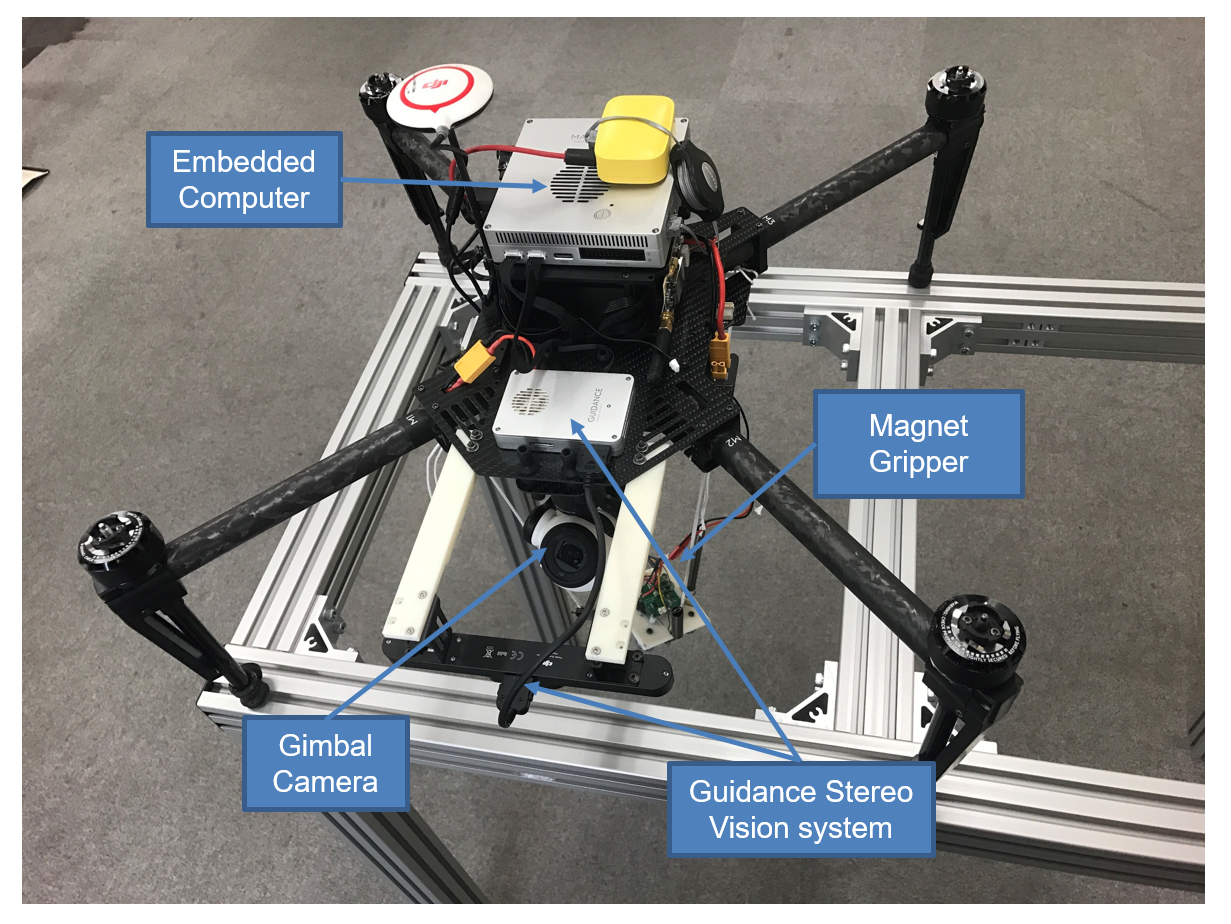
\includegraphics[keepaspectratio=true, width=1\linewidth, height=0.3\textheight]
    {sections//task3//images//task3platform.png}
      \end{center}
    \caption{Task 3 Platform: DJI M100}
    \label{task3platform-m100}
    \end{figure}
 \begin{figure}%[hb]
    \begin{center}
      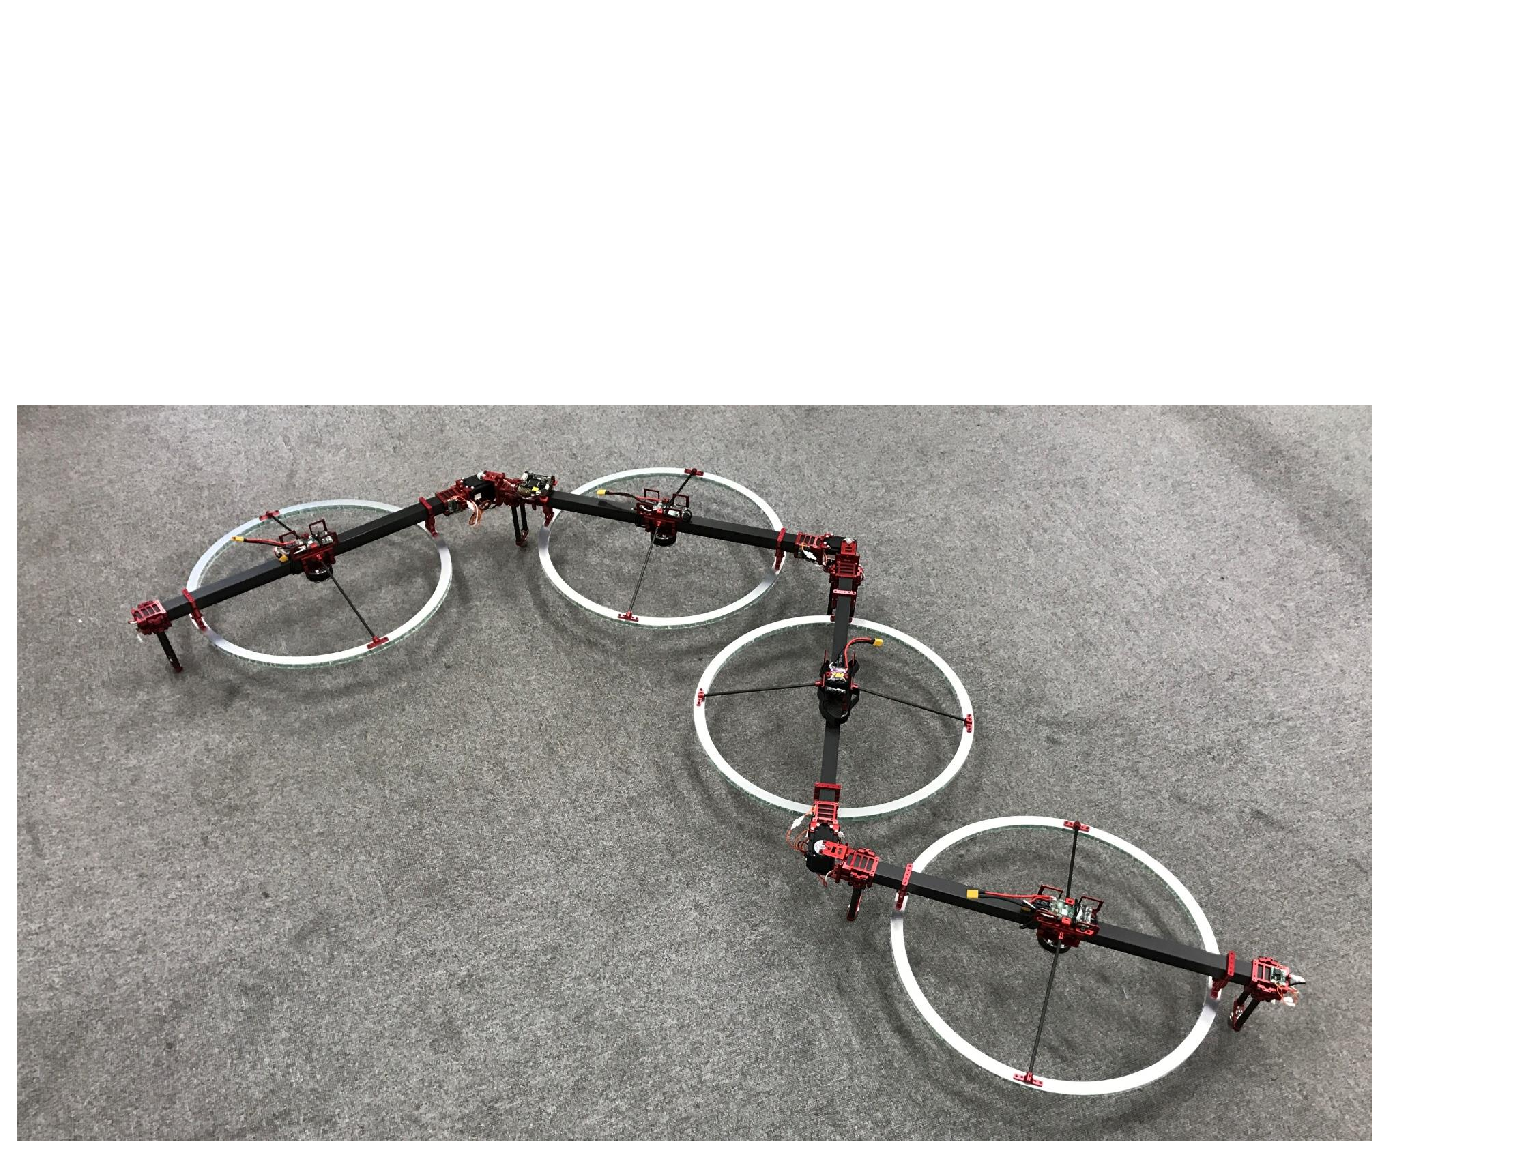
\includegraphics[clip, bb= 0 0 650 350, width=\columnwidth]{sections/task3/images/task3platform-hydrus.eps}
      \end{center}
    \caption{Task 3 Platform: Hydrus}
    \label{task3platform-hydrus}
    \end{figure}
    
    
\subsection{Electromagnet Gripper for Quadcopter}

The choice of electromagnet is based on easy control and also the circuits
can readily be designed by ourselves. The ordinary once are stronger but it
requires executor unit to push the object for releasing, which will
make the attachment more complex and may also require an additional motor. We
also contemplated to use a air vacuum but the size of vacuum is too
big for our drone.

 \begin{figure}[hb]
    \begin{center}
    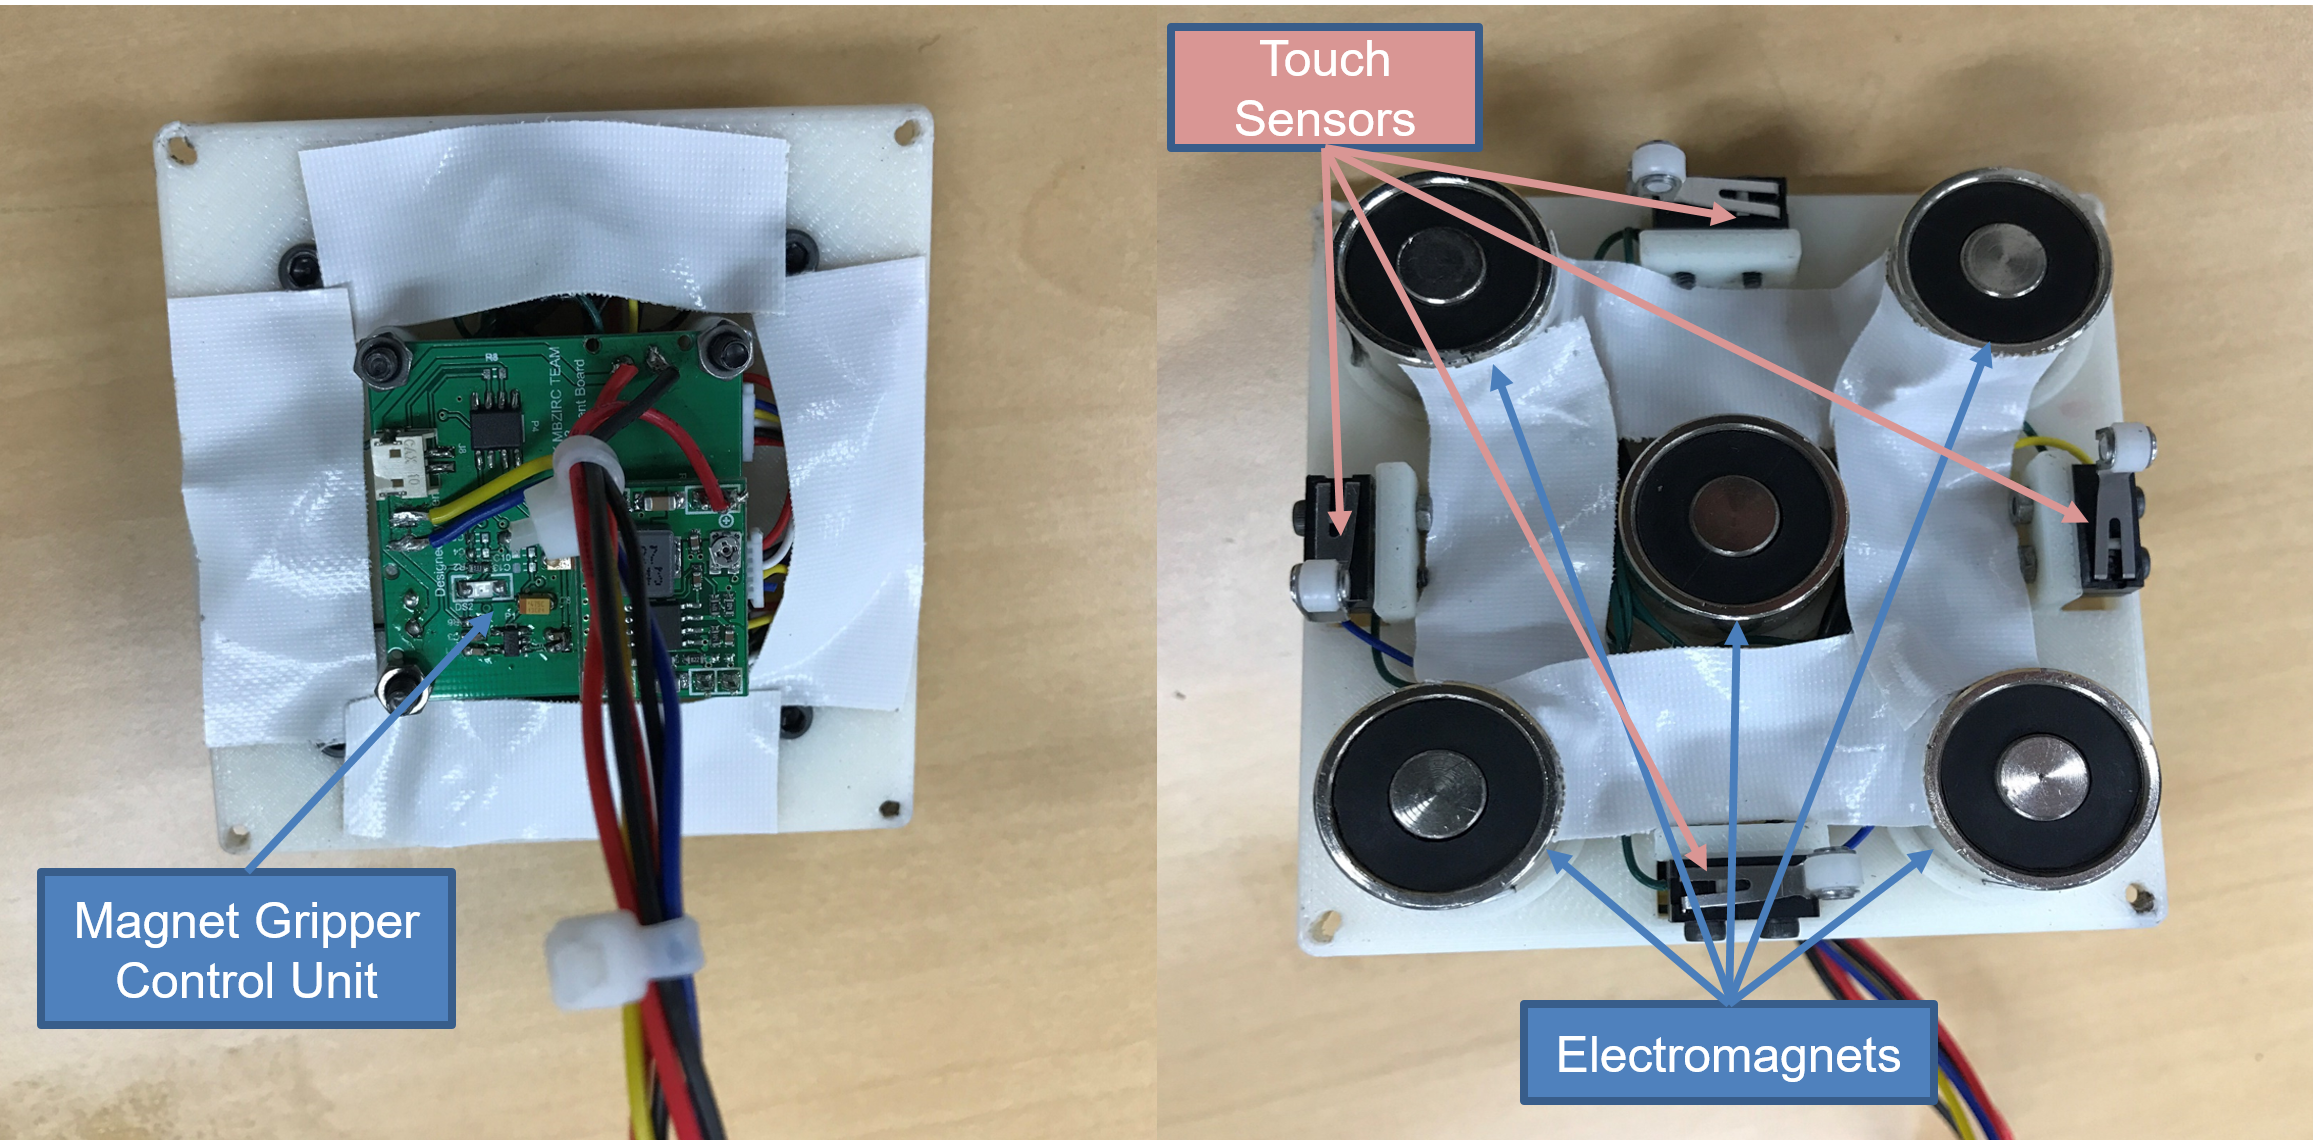
\includegraphics[keepaspectratio=true, width=1\linewidth, height=0.3\textheight]
    {sections//task3//images//task3gripper.png}
      \end{center}
    \caption{Task 3 Gripper($8cm \times 8cm, 240g$)}
    \label{task3platform}
    \end{figure}

We equipped 5 small electromagnets on a gripper of size $8cm \times
8cm$. Each electromagnet is capable of more withstanding than $20 N$
of force given a good object thickness. The gripper shown in
Fig.\ref{task3platform} consisting of $5$
electromagnets can pick the object of almost $1kg$ of the thickness of
the iron is more than $0.3mm$.
The gripper is also equipped with four touch sensors to detect
object--gripper contact state. Moreover,
these touch sensors are used to evaluate the position of the gripper
with respect to the object and the relative offset. 
%% For instance if $2$ or $3$ touch sensors
%% are triggered and then we know the offset of the gripper and the
%% object. 

%% However, according to our experiment,
%% since each object is less than $500 g$, the thickness will be less
%% than $1.6 mm$ if the object is a square of $20cm \times 20cm$ and made
%% of pure iron(consider the density of iron to be $7.86 g/cm$). 
%% In
%% addition, if the surface of the object is too large, the propeller
%% effect will happen and therefore request the electromagnets to be more
%% powerful. Temporary our gripper with $5$ electromagnets can pick the
%% object of almost $1kg$ of the thickness of the iron is more than
%% $0.3mm$. 


 \begin{figure*}%[hb]
    \begin{center}
    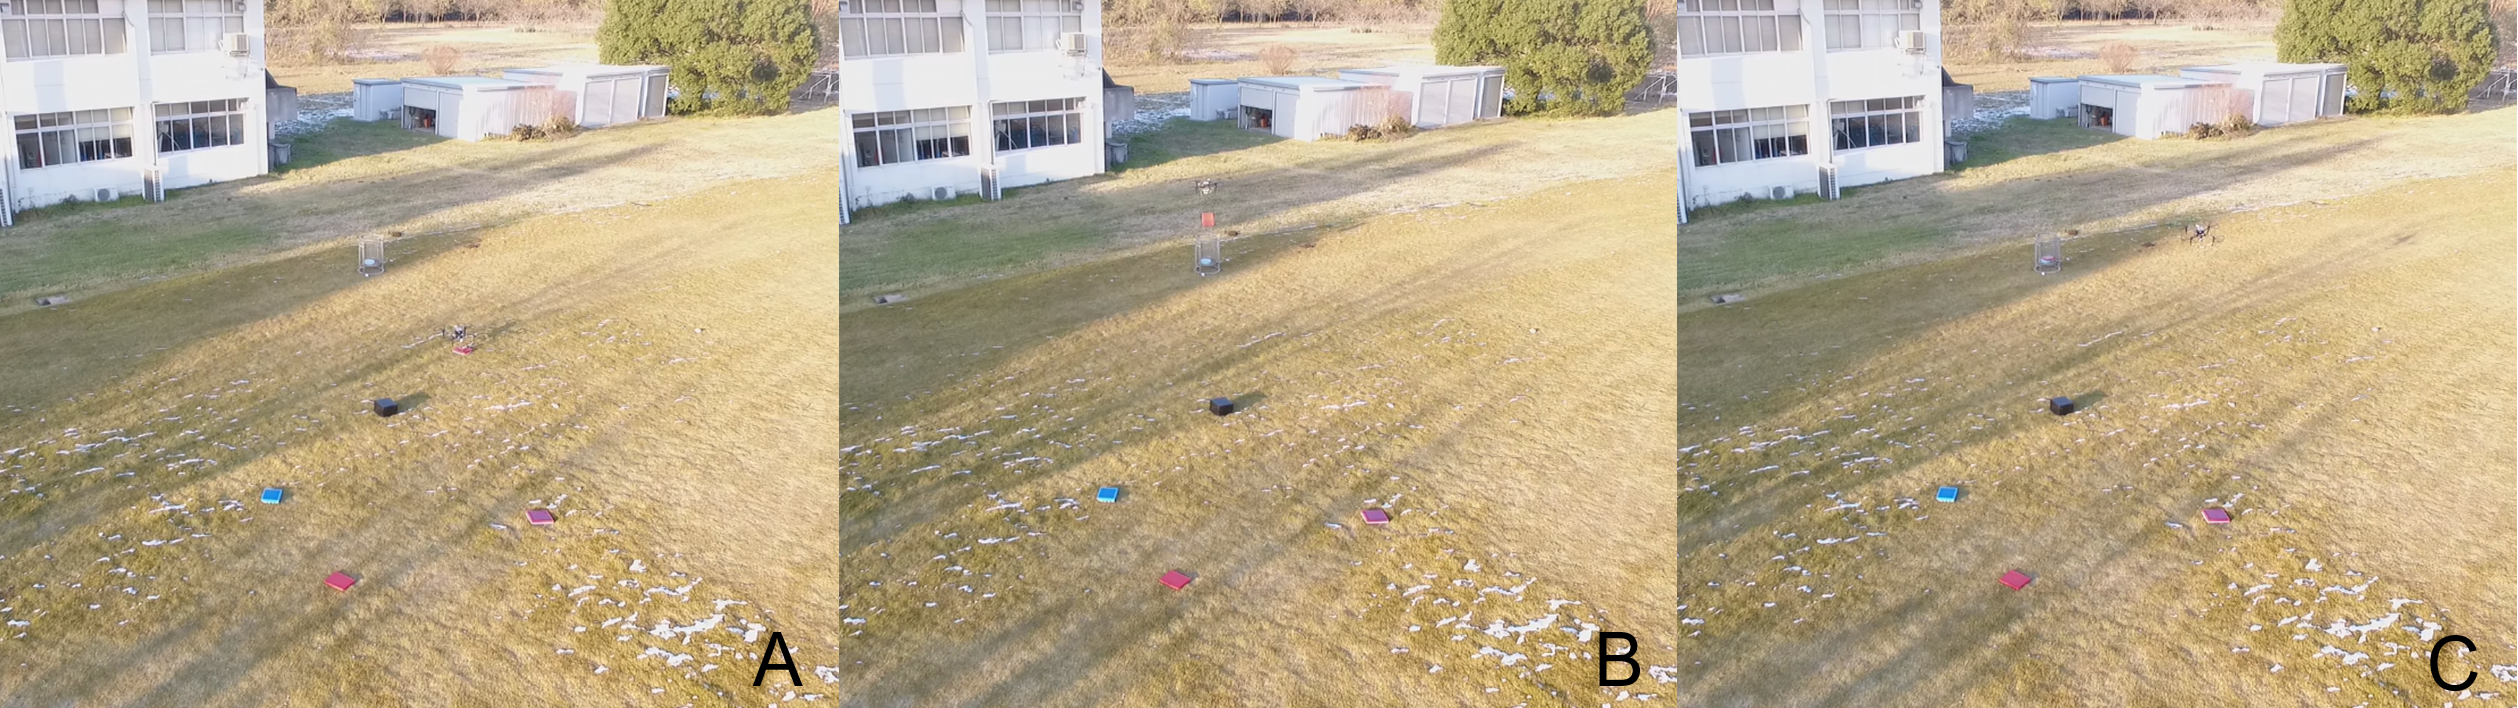
\includegraphics[keepaspectratio=true, width=1\linewidth, height=0.3\textheight]
    {sections//task3//images//teleop.png}
      \end{center}
    \caption{Pick, Place and Search in Teleoperation(A: Pick an object, B: Place the object back to a tray box, C: Search and approach to an object)}
    \label{task3tele}
    \end{figure*}

    
The design of the electromagnet circuits driver is simple since it can
be simply regarded as a series connection of a inductor and a small
resistor. Darlington Transistor is suitable to drive an
electromagnet as the current requirement is only $200 ma$. Because of
the inductor effect, a protection diode is necessary in the
circuits to prevent backflow. We designed the circuits board with a
$32$ bits micro controller, a Darlington driver IC and both serial, CAN communication
interface in the gripper board. An on board driver written on ROS node
collects the status of the magnets and the touch sensors in the
gripper and reports these information to the embedded computers.

%% on board driver written on ROS
%% the status of the magnets and the touch sensors in the gripper can be
%% collected and reported 
%% it can directly report the status of the magnets and touch sensors in
%% the gripper and also receive the orders from the embedded computers. 


\subsection{Teleoperation for Task 3}

We performed experiments using the aforementioned hardware interfaced
on the UAV. The UAVs were controlled through tele--operation. The
software which were implemented on the simulator needs
fine-tuning to operate in the real world. Approaching the object for
grasping is relatively difficult due to rapid visual changes. A more
crucial problem when approaching the object is the ground effect which 
results in unexpected behaviour and the UAV becomes unstable very
quickly. We addressed this problem by suspending the magnet gripper with
a spring so that the UAV can pick the object without getting too close
to the ground. However this introduces another problem i.e., causes
the gripper to shake whenever the UAV change the velocity. We are
currently working towards alleviating the problem.



%% When we control the UAV manually to
%% pick the object, we figure out it is not a easy job for real UAV
%% platform compared to the simulation since it is very difficult to
%% control the UAV accurately to approach the object, in addition, the
%% ground effect will unstable the UAV when the UAV is getting close to
%% the ground. We address this problem by hanging the magnet gripper with
%% a spring so that the UAV can pick the object without getting too close
%% to the ground. However this may introduce another problem that the
%% gripper will be shaking whenever the UAV change the velocity, we are
%% also addressing this problem now and try to get a stronger hanging
%% method to make the gripper relatively stable.

%% At this moment, we only perform the real platform experiment through
%% teleoperation by human beings. When we control the UAV manually to
%% pick the object, we figure out it is not a easy job for real UAV
%% platform compared to the simulation since it is very difficult to
%% control the UAV accurately to approach the object, in addition, the
%% ground effect will unstable the UAV when the UAV is getting close to
%% the ground. We address this problem by hanging the magnet gripper with
%% a spring so that the UAV can pick the object without getting too close
%% to the ground. However this may introduce another problem that the
%% gripper will be shaking whenever the UAV change the velocity, we are
%% also addressing this problem now and try to get a stronger hanging
%% method to make the gripper relatively stable.

\subsection{Results}

We performed experiments using one UAV i.e., the standard platform. 
%We tested on one UAV and it seems 
On average we can pick $5$ static objects within $8$ minutes, the time
could be improved if we adopt the
semi-autonomous teleoperation method like store the global position of
the box to drop the objects and after picking the object, the UAV can
directly move to the global position of the drop box.


\subsection{Future Work}
In the next step of task 3 we are going to improve our vision
detection method. While the performance of these algorithms yield good
results in simulation, they still need improvements when applying to
the real world. With improvements in the vision algorithms and reduced
in gripper shakes we will make the task3 fully autonomous 
Also we will design a multi UAVs cooperation strategy for
task 3 both for teleoperation and full autonomous.


\end{document}


\section{GRAND CHALLENGE}

%Copyright (C) 2016 by Krishneel@JSK Lab, The University of Tokyo

\documentclass{standalone}

\usepackage{graphicx}
\usepackage{float}
\floatstyle{boxed} 
\restylefloat{figure}

\begin{document}

\subsection{Setup of Testbed}
We have started to operate all tasks simultaneously, as shown in Fig.\ref{fig:grand}. The fundamental performances of each task have been comfirmed.

 \subsection{Future Work}
We plan to establish the mutual communication among the filed robots to enhance the performance. For instance, we will use the image data from the robot of task2 to recognize the truck of task1 and objects of task3, and vice versa.
 
\begin{figure}[h]
    \begin{center}
      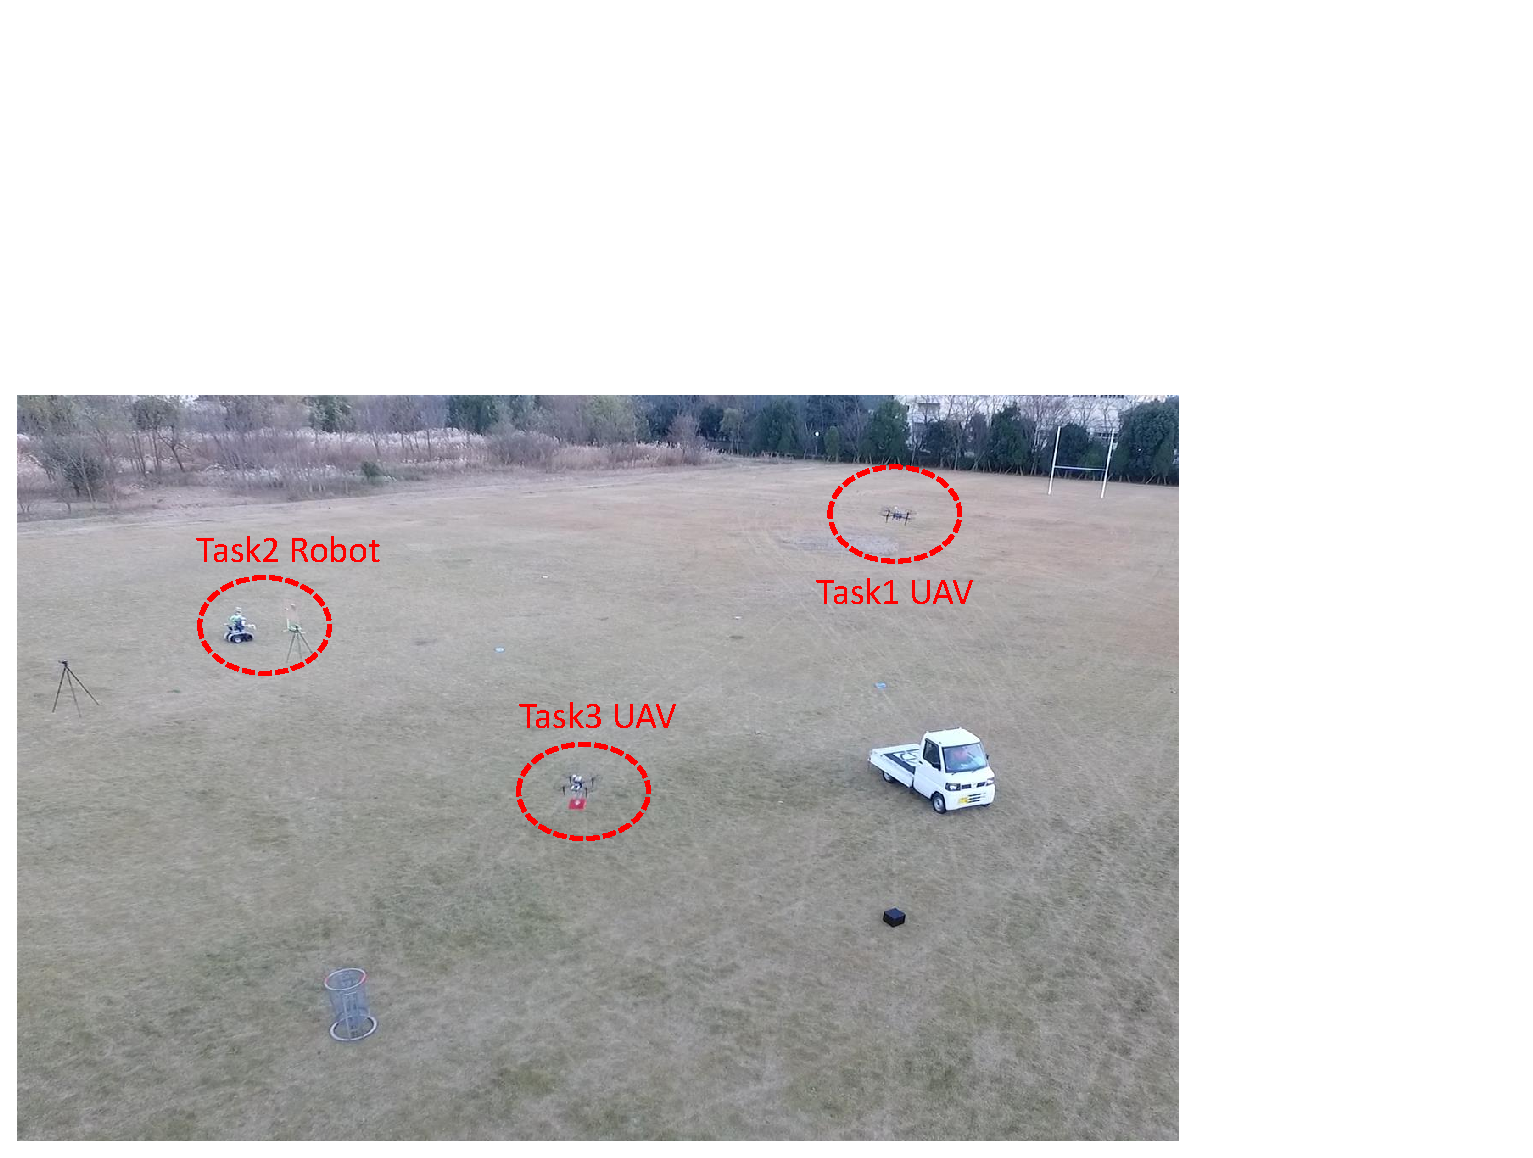
\includegraphics[clip, bb= 0 0 560 360, width=1.0\columnwidth]{sections/grand/images/grand_challenge.eps}
    \end{center}
   \caption{Experiment of Ground Challenge in Kasihiwa, Chiba, Japan}
   \label{fig:grand}
 \end{figure}


\end{document}


%\section{Future Plan}

\end{document}
